\documentclass[polish,11pt,a4paper]{article}
\usepackage[utf8]{inputenc}
\usepackage[T1]{fontenc}
\usepackage{graphicx}
\usepackage{amsfonts}
\usepackage{amssymb}
\usepackage{graphicx}
\usepackage{svg}
\usepackage[utf8]{inputenc}
\usepackage{tikz}
\usepackage{tabularx}
\usepackage[centertags]{amsmath}
\usepackage{amsthm}
\usepackage{newlfont}
\usepackage[polish]{babel}
\usepackage[T1]{fontenc}
\usepackage{listingsutf8}
\usepackage{xcolor}
\usepackage{url}
\usepackage[autostyle]{csquotes}
\usepackage[T1]{fontenc}
\usepackage[utf8]{inputenc}
\usepackage{babel}
\usepackage[labelsep=period]{caption}

\usepackage{hyperref}
\hypersetup{
    colorlinks,
    citecolor=black,
    filecolor=black,
    linkcolor=black,
    urlcolor=black
}

\fontsize{12}{15}

\title{\huge{Model konceptualny}}
\author{\large{Oskar Tołkacz, 291583}}


\begin{document}

\clearpage
\maketitle
\thispagestyle{empty}

\newpage
\tableofcontents

\newpage

\section{Diagram ER}
\begin{center}
	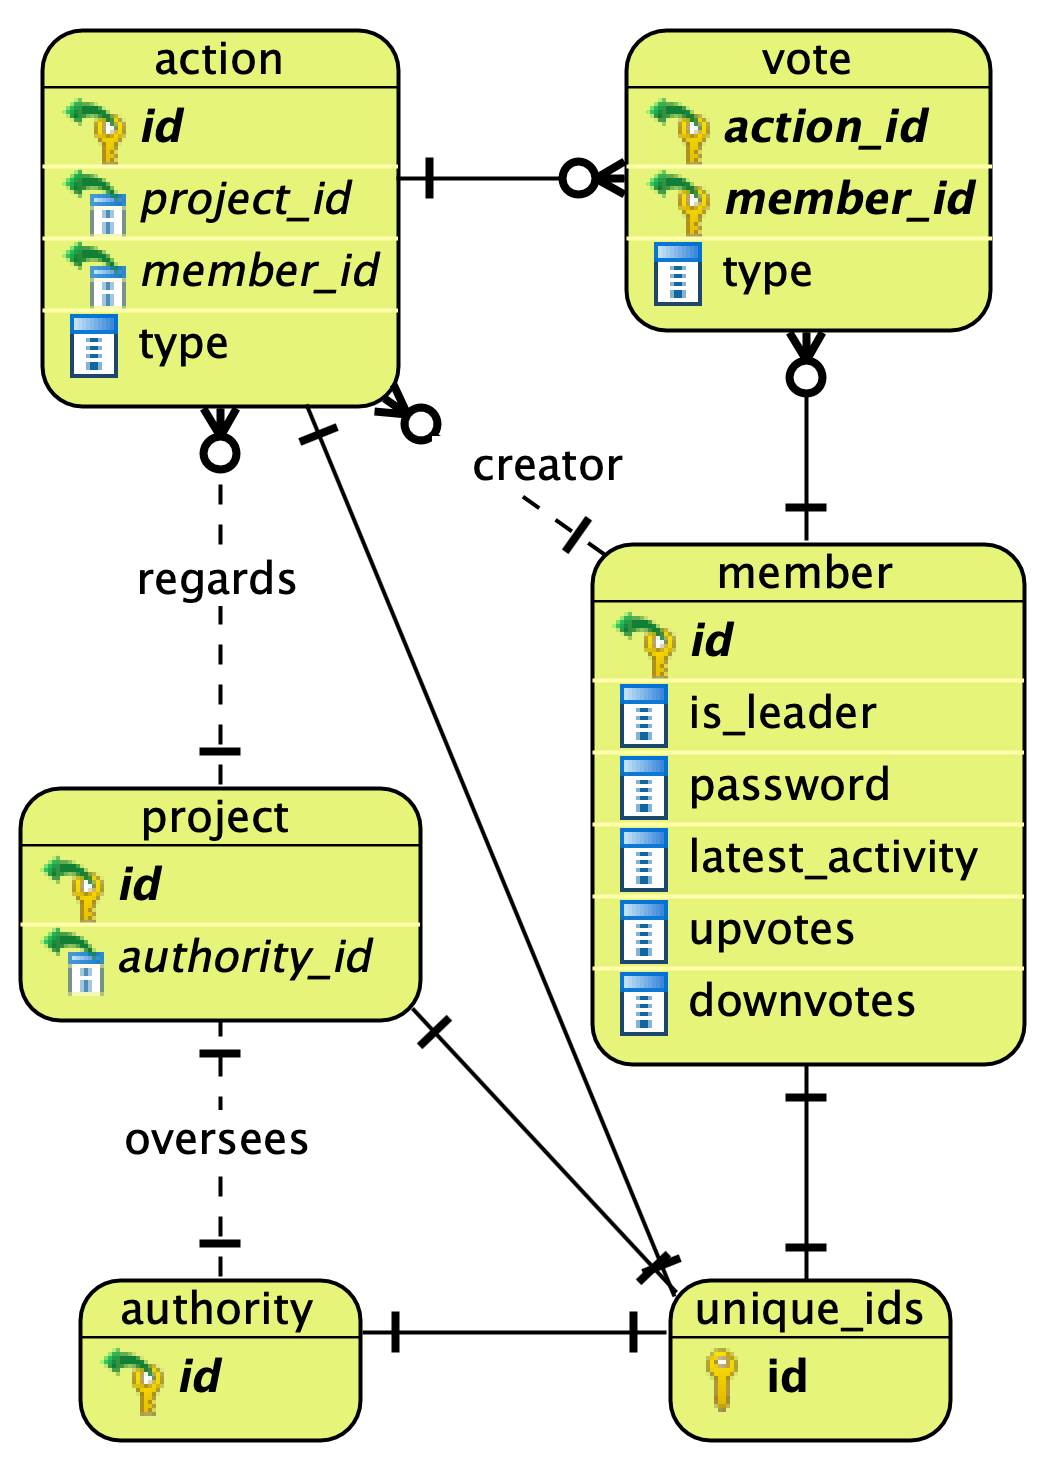
\includegraphics[scale=0.3]{ERD.png}
\end{center}

\section{Dodatkowe więzy}
\begin{itemize}
    \item Wartości w kolumnie \texttt{member(latest\_activity)} są timestampami ostatnich aktywności członków partii.
    \item Kolumna \texttt{member(upvotes)} jest sumą głosów za dla wszystkich akcji danego członka partii. Analogicznie dla kolumny \texttt{member(downvotes)} oraz głosów przeciwko.
\end{itemize}

\section{Uprawnienia użytkowników}
    \subsection{init}
        Ma pełne uprawnienia.
    \subsection{app}
        Może tylko odwoływać się do funkcji zdefiniowanych w API.

\section{Implementacja API}

    \subsection{open}
        Otwiera połączenie z bazą danych przy pomocy biblioteki Psycopg2. Wykonuje polecenia SQL dodające użytkownika \texttt{app} z odpowiednimi uprawnieniami oraz tworzące wszystkie potrzebne tabele, wyzwalacze, więzy, funkcje, itp.

    \subsection{leader}
        Dodaje rekord do tabeli \texttt{member} z polem \texttt{is\_leader} równym: true. Identyfikator nowego członka jest dodawany najpierw do tabeli \texttt{unique\_ids}. Podobnie będzie w przypadku dodawania akcji, projektów i organów władzy, Wymusza to globalną unikalność tych identyfikatorów.

    \subsection{support}
        Sprawdzane jest czy użytkownik dodający akcję nie jest zamrożony. Jeśli jest, to operacja jest przerywana. W przeciwnym przypadku dodawana jest nowa akcja. Najpierw tworzone są wszelkie potrzebne klucze, podobnie jak w przypdaku dodawania lidera. 
    \subsection{protest}
        Analogicznie jak \texttt{support}.

    \subsection{upvote}
        Dodawany jest nowy rekord to tabeli \texttt{votes}. Więzy wymuszają odpowiednie zachowanie bazy danych w przypadku, gdy akcja na którą będzie oddany głos nie będzie istaniała lub ten sam członek partii odda dwa głosy.
    \subsection{downvote}
        Analogicznie jak \texttt{upvote}.

    \subsection{actions}
        Wynikiem będzie pogrupowane po akcjach złączenie tabel: \texttt{action} oraz \texttt{vote}. Należy uwzględnić opcjonalne parametry określające sposób filtrowania po typie akcji, identyfikatorze działania czy identyfikatorze organu władzy.
        
    \subsection{projects}
       Należy zwrócić tabelę \texttt{project}, po ewentualnym pofiltrowaniu w przypadku otrzymania identyfikatora organu władzy. 
        
    \subsection{votes}
        Wynikiem będą kolumny z odpowiednio pogrupowanej tabeli \texttt{member} złączonej z tabelą \texttt{vote}. W przypdaku otrzymania odpowiedniego argumentu określającego projekt, tabele będzie trzeba złączyć dodatkowo z tabelą \texttt{project}.

    \subsection{trolls}
        Wystarczy wziąć dane z tabli \texttt{member} i odrzucić członków którzy mają więcej głosów za niż przeciw oraz posortować.
    
\end{document}
